\documentclass[11pt]{beamer}
\usetheme{Warsaw}
\usepackage[utf8]{inputenc}
\usepackage[english]{babel}
\usepackage{amsmath}
\usepackage{amsfonts}
\usepackage{amssymb}
\usepackage{color}
\usepackage{graphicx}
\definecolor{gray}{gray}{0.55}
\author{\textcolor{gray}{Adel Benamara} \and \underline{Thomas Gougeon} \and \underline{Ludovic
Robin}}
\title{Library version checking - QuarksLab}
%\setbeamercovered{transparent} 
%\setbeamertemplate{navigation symbols}{} 
%\logo{} 
%\institute{} 
%\date{} 
%\subject{} 
\begin{document}

\begin{frame}
\titlepage
\end{frame}

\begin{frame}
\tableofcontents
\end{frame}

\section{Introduction}
\begin{frame}{Introduction}

    \begin{center}
    
\includegraphics[scale=0.38]{hacker.png}
    \end{center}

    \begin{block}{}
        \begin{itemize}
            \item \underline{Hackers} look for vulnerabilities in programs ;
            \item Sometimes, finding one allow them to make an exploit ;
            \item \underline{Developers} try to fix vulnerabilities, publishing a patch ;
            \item \underline{Users} install the patch to hopefully fix the vulnerability on
                their version of the program.
        \end{itemize}
    \end{block}
\end{frame}

\begin{frame}
    \frametitle{What could go wrong ?}
    \begin{center}
    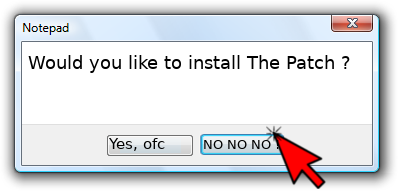
\includegraphics[scale=0.5]{box.png}
    \end{center}

    \begin{block}{}
    \begin{itemize}
        \item The vulnerability is not necessarily patched and the old version may remain ;
        \item \Huge Very \textcolor{red}{dangerous} !
    \end{itemize}
    \end{block}

    \end{frame}
\begin{frame}
    \begin{block}{Problem}
        \begin{itemize}
            \item How do we know if a library is patched ?  
            \item How to check if we applied a patch ?
        \end{itemize}
    \end{block}
   

    Let L be the library
        En entree on a une librairie binaire en .so et on va repondre a la
        question: Quelle est la version de cette librairie?

        Du coup on nous donne un .so 
        Et on a pleiun de sources de librairies connues

        Dans la suite on va considerer que la librairie binaire a ete compilee
        dans la meme architecture que notre machine 
\end{frame}


\begin{frame}

    Approche naive, on compile nos librairies et les compare bit par bit avec
    L

    Probleme: L est compile avec un compilateur different et des options de
    ocmpilations differentes.

    Les binaires sont trop differents, meme si ils font potentiellement la
    meme chose.

\end{frame}

\begin{frame}

    Il faut trouver des methodes plus intelligentes pour comparer les
    binaires.

    \begin{itemize}
        \item Linkage 
        \item Malware signature
        \item Traces
    \end{itemize}

\end{frame}

\begin{frame}
    \frametitle{Link dynamically the library}
    blabla  
\end{frame}

\begin{frame}
    \frametitle{Malware signature}
\end{frame}

\begin{frame}
    \frametitle{Analyse traces} 
\end{frame}

\begin{frame}
    \begin{block}{Context}


    \end{block}

    \begin{block}{Fred's problems}

        \begin{itemize}
            \item Libraries version
            \item Find other execution paths for a root cause
        \end{itemize}

    \end{block}

\end{frame}

\section{Find library version}
\begin{frame}{Find library version automatically}

    \begin{block}{Objective}
        \begin{itemize}
            \item Given a binary lib $L$ used in a program $P$
            \item What is the version of $L$ ?
            \item A database $D$ of sources of all the version is available
        \end{itemize}
    \end{block}

    \begin{block}{Motivation}
        \begin{itemize}
            \item Programs often use old libraries
            \item These libraries include known vulnerabilities
        \end{itemize}
    \end{block}

    \begin{block}{Issues}
        \begin{itemize}
            \item Manual investigation is not trivial (strings, calls, \dots)
            \item Only $2$ persons in the team (who is Adel ?)
        \end{itemize}

    \end{block}

\end{frame}


\begin{frame}{First approaches}

\begin{block}{Compare binaries}
	\begin{itemize}
		\item Compare the binary code of $L$ with binaries generated by the sources of $D$
		\item Compare a signature of $L$ with a signature of $D$ (CFG ?)
		\item Compare the symbol list of $L$ with those of $D$
	\end{itemize}
\end{block}

\begin{block}{Issues}
	\begin{itemize}
		\item Binaries, CFG, and symbols depend on the architecture compilation target and the compiler version
		\item Binaries, CFG, and symbols depend on the source code
		\item How to detect if the difference comes from the patch or the compilation ?
	\end{itemize}
\end{block}

\end{frame}



\begin{frame}{Second approaches}

\begin{block}{Compare execution}
	\begin{itemize}
		\item Compare traces of execution from $L$ to those of $D$ 
		\item Compare signatures of functions
		\item Call functions with NULL arguments
	\end{itemize}
\end{block}

\begin{block}{Issues}
	\begin{itemize}
		\item How to call functions of $L$ ? Sometimes there are tests
		\item Differentiate only major versions
		
	\end{itemize}
\end{block}


\end{frame}

\begin{frame}{Toy example}

Mettre un exemple pour montrer comment ca marche cette idee


\end{frame}

\begin{frame}{Automating}
\begin{block}{Scripts in Perl}
\begin{itemize}
	\item Generate headers from sources
	\item Generate so from sources
	\item Generate test.c
\end{itemize}

\end{block}

\end{frame}



\begin{frame}{Differentiate minor versions}

\begin{block}{Heuristics}
	\begin{itemize}
		\item Compare CFG of functions
		\item 
	\end{itemize}
\end{block}

\end{frame}

\begin{frame}{Further ideas}

\begin{block}


\end{block}

\end{frame}


\begin{frame}{Find other root paths}
\begin{block}{Coccinelle}
	\begin{itemize}
		\item Find known bugs in source code
		\item Analyse patterns in source
		\item Issue: We deal with binaries
		\item Useful to find other execution paths for root cause
	\end{itemize}
\end{block}
\end{frame}





\section{Conclusion}


\begin{frame}{Conclusion}

	\begin{block}{Issues}
		\begin{itemize}
			\item Adel leaves us alone
			\item A lot of tools do nothing
		\end{itemize}
	
	\end{block}
	\begin{block}{Results}
		\begin{itemize}
			\item Differentiate major versions =
		\end{itemize}
		
	\end{block}
\end{frame}

\begin{frame}{Organisation}

\begin{block}{Tools and communication}
\begin{itemize}
	\item GitHub
	\item IRC
	\item Audio meetings
\end{itemize}
\end{block}

\begin{block}{Agility}
	\begin{itemize}
		\item Separation in tasks
		\item Meetings every hour
	\end{itemize}
\end{block}


\end{frame}

\begin{frame}{It brought us..}


\begin{block}{Mind}
	\begin{itemize}
		\item Inner peace
		\item Happiness
	\end{itemize}
\end{block}

\begin{block}{Technical}
	\begin{itemize}
		\item Perl/Bash
		\item Binaries
		\item Compilation
	\end{itemize}
	
\end{block}

\end{frame}
\end{document}
